\section{Jagt fra kunstige skjul}

\begin{frame}
  \vspace{3em}
  \begin{center}
    {\LARGE \textbf{Jagt fra kunstige skjul}
    }
    \\
    \vspace{1em}
    Bekendtgørelse om udsætning af vildt, jagtmåder og jagtredskaber
    \\
    \vspace{1em}
    BEK nr 1652 af 19/12/2017, Kapitel 1
  \end{center}
\end{frame}

\begin{frame}
    \frametitle{Forbud mod jagt på pattedyr fra kunstige skjul (§ 1)}

    \vspace{1.5cm}

    § 1

    \vspace{0.5cm}

    Der må ikke drives jagt på pattedyr fra

    \vspace{0.5cm}

    1) kunstigt skjul, herunder hus, hytte, jordhul, eller

    \vspace{0.5cm}

    2) platform eller sæde, der er hævet mere end 50 cm over det omgivende terræn.

    \vspace{0.5cm}

    Med to undtagelser

    \vspace{2.5cm}
\end{frame}

\begin{frame}
    \frametitle{Varianter af kunstige skjul}

    \begin{columns}
        \column{0.5\textwidth}
        \centering
        \begin{figure}
            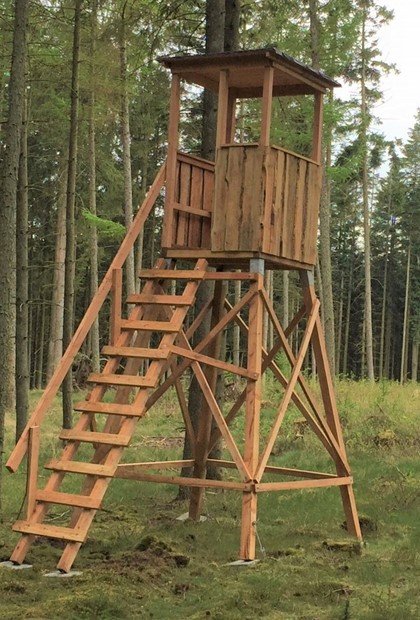
\includegraphics[width=0.5\textwidth]{Billeder/Redskaber/jagttårn.jpg}
            \caption{\textbf{Jagttårn} (jægeren kan skyde stående)}
        \end{figure}
        
        \column{0.5\textwidth}
        \centering
        \begin{figure}
            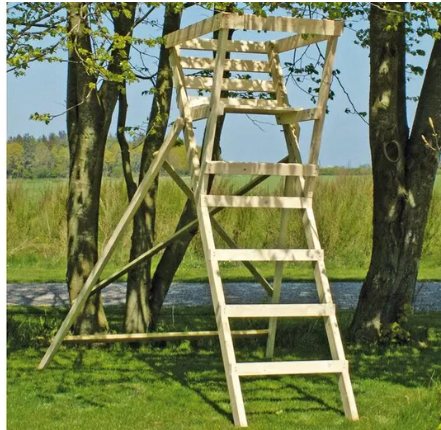
\includegraphics[width=0.5\textwidth]{Billeder/Redskaber/jagtstige.png}
            \caption{\textbf{Jagtstige} (jægeren kan skyde siddende)}
        \end{figure}
    \end{columns}

    \vspace{1cm}  % Plads til tekst under

    \centering
\end{frame}

\begin{frame}
    \frametitle{Regler for skydetårne (§ 1)}

    \begin{columns}[T]  % T for top-alignment
        \column{0.6\textwidth}
        \begin{itemize}
            \item Højere end 50 cm over omkringliggende areal
            \item Min 130 m til skel med mindre andet er aftalt skriftligt
            \item Udført i træ eller metal
            \item Opsættes i min 0,5 hektar skov eller ydre/inde skovbryn
            \item Må ikke skæmme (samme højde som øvrig bevoksning)
            \item Højde til plateau max 5m
            \item Sider max 110cm høje
            \item Plateau max 2 $m^2$
            \item Tag i et plan, ikke-reflekterende, max 10 cm udhæng
        \end{itemize}
        
        \column{0.4\textwidth}
        \centering
        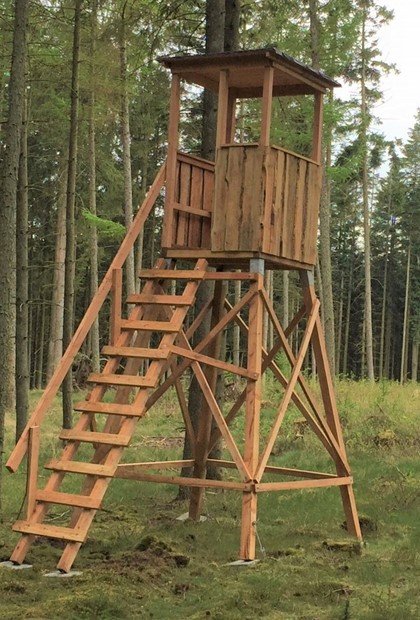
\includegraphics[width=0.7\textwidth]{Billeder/Redskaber/jagttårn.jpg}  % Mindre billede nu
        \vspace{0.5cm}
        \small 
    \end{columns}

\end{frame}

\begin{frame}
    \frametitle{Regler for skydestiger (§ 1)}

    \begin{columns}[T]  % T for top-alignment
        \column{0.6\textwidth}
        \begin{itemize}
            \item Højere end 50 cm over omkringliggende areal
            \item Min 130 m til skel med mindre andet er aftalt skriftligt
            \item De skal være mobile eller midlertidige konstruktioner
            \item Opsættes i hegn eller bevoksninger (ikke 0,5 hektar regel)
            \item Må ikke skæmme (samme højde som øvrig bevoksning)
            \item Højde til plateau max 5 m
        \end{itemize}
        
        \column{0.4\textwidth}
        \centering
        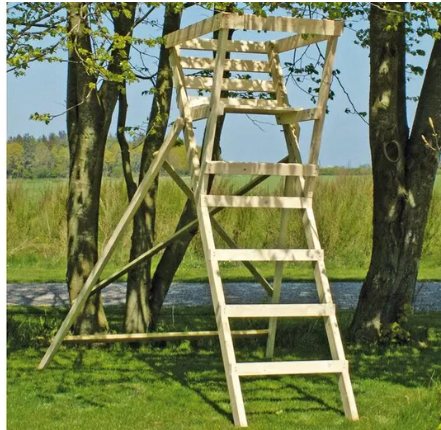
\includegraphics[width=0.7\textwidth]{Billeder/Redskaber/jagtstige.png}  % Mindre billede nu
        \vspace{0.5cm}
        \small 
    \end{columns}

    \end{frame}

\begin{frame}
    \frametitle{Regler for kunstige skjul på fugle (§ 3)}

    \begin{columns}[T]  % T for top-alignment
        \column{0.6\textwidth}
        \begin{itemize}
            \item Gulvet/ståstedet må højest være hævet 50 cm over terrænnet
            \item Ellers er kreativiteten ubegrænset – brug camouflage, net, siv, grene osv.
            \item Skjulet kan være midlertidigt (flytbart) eller mere fast (f.eks. ramme med net)
            \item Ofte brugt til andejagt, duejagt eller kragejagt med lokkefugle
            \item Husk at våbentype skal passe til skjulet (typisk haglgevær til fugle) (§ 2)
            \item Skjulet skal camouflages godt for ikke at skræmme vildtet
        \end{itemize}
        
        \column{0.4\textwidth}
        \centering
        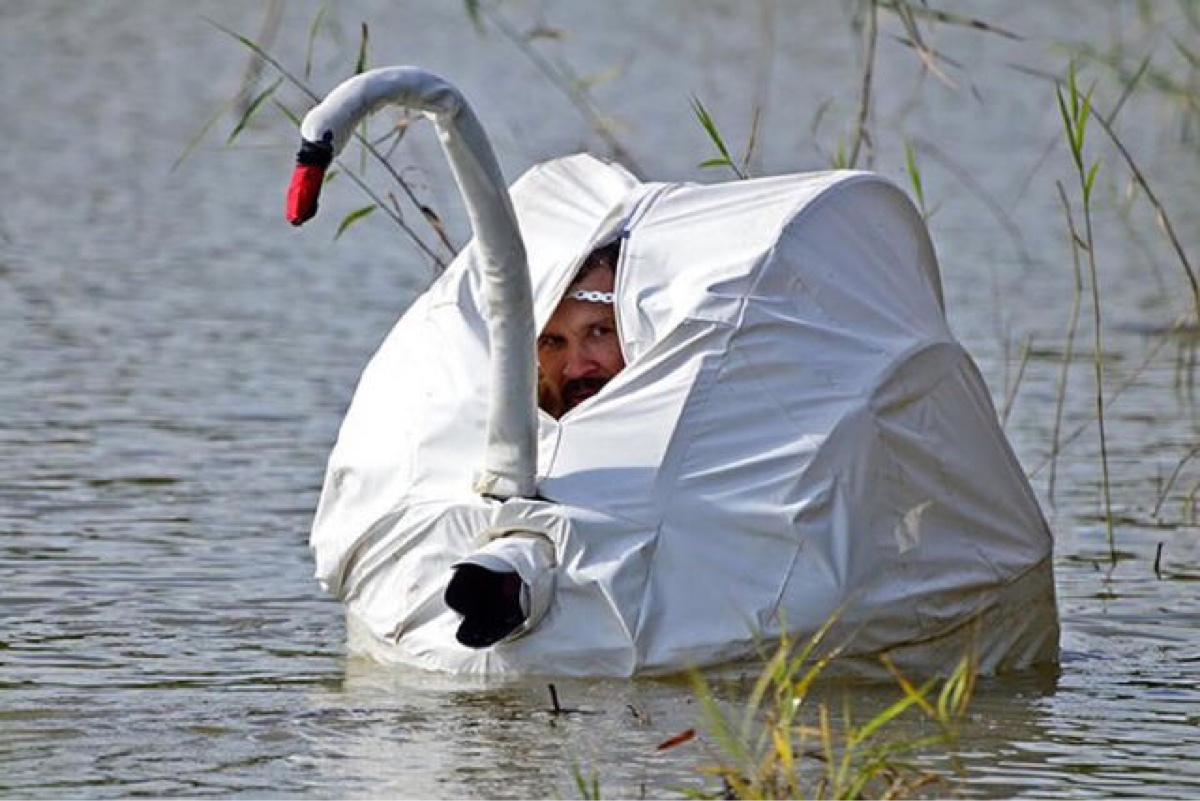
\includegraphics[width=0.9\textwidth]{Billeder/Redskaber/kunstigtskjul.jpg}
        \vspace{0.5cm}
        
    \end{columns}

\end{frame}
